%% Copernicus Publications Manuscript Preparation Template for LaTeX Submissions
%% ---------------------------------
%% This template should be used for copernicus.cls
%% The class file and some style files are bundled in the Copernicus Latex Package, which can be downloaded from the different journal webpages.
%% For further assistance please contact Copernicus Publications at: production@copernicus.org
%% https://publications.copernicus.org/for_authors/manuscript_preparation.html


%% Please use the following documentclass and journal abbreviations for preprints and final revised papers.

%% 2-column papers and preprints
\documentclass[journal abbreviation, manuscript]{copernicus}


%% Journal abbreviations (please use the same for preprints and final revised papers)

% Advances in Geosciences (adgeo)
% Advances in Radio Science (ars)
% Advances in Science and Research (asr)
% Advances in Statistical Climatology, Meteorology and Oceanography (ascmo)
% Aerosol Research (ar)
% Annales Geophysicae (angeo)
% Archives Animal Breeding (aab)
% Atmospheric Chemistry and Physics (acp)
% Atmospheric Measurement Techniques (amt)
% Biogeosciences (bg)
% Climate of the Past (cp)
% DEUQUA Special Publications (deuquasp)
% Earth Surface Dynamics (esurf)
% Earth System Dynamics (esd)
% Earth System Science Data (essd)
% E&G Quaternary Science Journal (egqsj)
% EGUsphere (egusphere) | This is only for EGUsphere preprints submitted without relation to an EGU journal.
% European Journal of Mineralogy (ejm)
% Fossil Record (fr)
% Geochronology (gchron)
% Geographica Helvetica (gh)
% Geoscience Communication (gc)
% Geoscientific Instrumentation, Methods and Data Systems (gi)
% Geoscientific Model Development (gmd)
% History of Geo- and Space Sciences (hgss)
% Hydrology and Earth System Sciences (hess)
% Journal of Bone and Joint Infection (jbji)
% Journal of Micropalaeontology (jm)
% Journal of Sensors and Sensor Systems (jsss)
% Magnetic Resonance (mr)
% Mechanical Sciences (ms)
% Natural Hazards and Earth System Sciences (nhess)
% Nonlinear Processes in Geophysics (npg)
% Ocean Science (os)
% Polarforschung - Journal of the German Society for Polar Research (polf)
% Primate Biology (pb)
% Proceedings of the International Association of Hydrological Sciences (piahs)
% Safety of Nuclear Waste Disposal (sand)
% Scientific Drilling (sd)
% SOIL (soil)
% Solid Earth (se)
% State of the Planet (sp)
% The Cryosphere (tc)
% Weather and Climate Dynamics (wcd)
% Web Ecology (we)
% Wind Energy Science (wes)


% \usepackage commands included in the copernicus.cls:
% \usepackage[german, english]{babel}
% \usepackage{tabularx}
% \usepackage{cancel}
% \usepackage{multirow}
% \usepackage{supertabular}
% \usepackage{algorithmic}
% \usepackage{algorithm}
% \usepackage{amsthm}
% \usepackage{float}
% \usepackage{subfig}
% \usepackage{rotating}
\usepackage{booktabs}
\usepackage{multirow}


\begin{document}

\title{TEXT}


% \Author[affil]{given_name}{surname}

\Author[][EMAIL]{}{} %% correspondence author
\Author[]{}{}
\Author[]{}{}

\affil[]{ADDRESS}
\affil[]{ADDRESS}

%% The [] brackets identify the author with the corresponding affiliation. 1, 2, 3, etc. should be inserted.

%% If an author is deceased, please mark the respective author name(s) with a dagger, e.g. "\Author[2,$\dag$]{Anton}{Smith}", and add a further "\affil[$\dag$]{deceased, 1 July 2019}".

%% If authors contributed equally, please mark the respective author names with an asterisk, e.g. "\Author[2,*]{Anton}{Smith}" and "\Author[3,*]{Bradley}{Miller}" and add a further affiliation: "\affil[*]{These authors contributed equally to this work.}".


\runningtitle{TEXT}

\runningauthor{TEXT}

\received{}
\pubdiscuss{} %% only important for two-stage journals
\revised{}
\accepted{}
\published{}

%% These dates will be inserted by Copernicus Publications during the typesetting process.


\firstpage{1}

\maketitle



\begin{abstract}
TEXT
\end{abstract}


\copyrightstatement{TEXT} %% This section is optional and can be used for copyright transfers.


\introduction  %% \introduction[modified heading if necessary]


\section{Data and Methods}

\subsection{Site and database}

An extensive dataset ranging the years 2018 to 2023 was used. In particular, Cloudnet \cite{Illingworth2007XXX} post-processed high level data
% data levels 1c and 2, 
and radiometer humidity and temperature profiles. These products were inferred by measurements carried out with a set of ground-based remote sensing instruments - managed at the ACTRIS-CCRES Granada site facility (CCRES stands for Centre for Cloud Remote Sensing) at 37$^{\circ}$2E, 3.6$^{\circ}$S and 680 m, Southeast Spain. This station is as part of the University of Granada (UGR) and it is integrated into the AGORA observatory. Figure \ref{fig:granada_station} shows the station, located within a broad intramontane depression in the foothills of the tallest mountain massif of the Iberian Peninsula, Sierra Nevada. 

\begin{figure}[htbp]
      \centering
      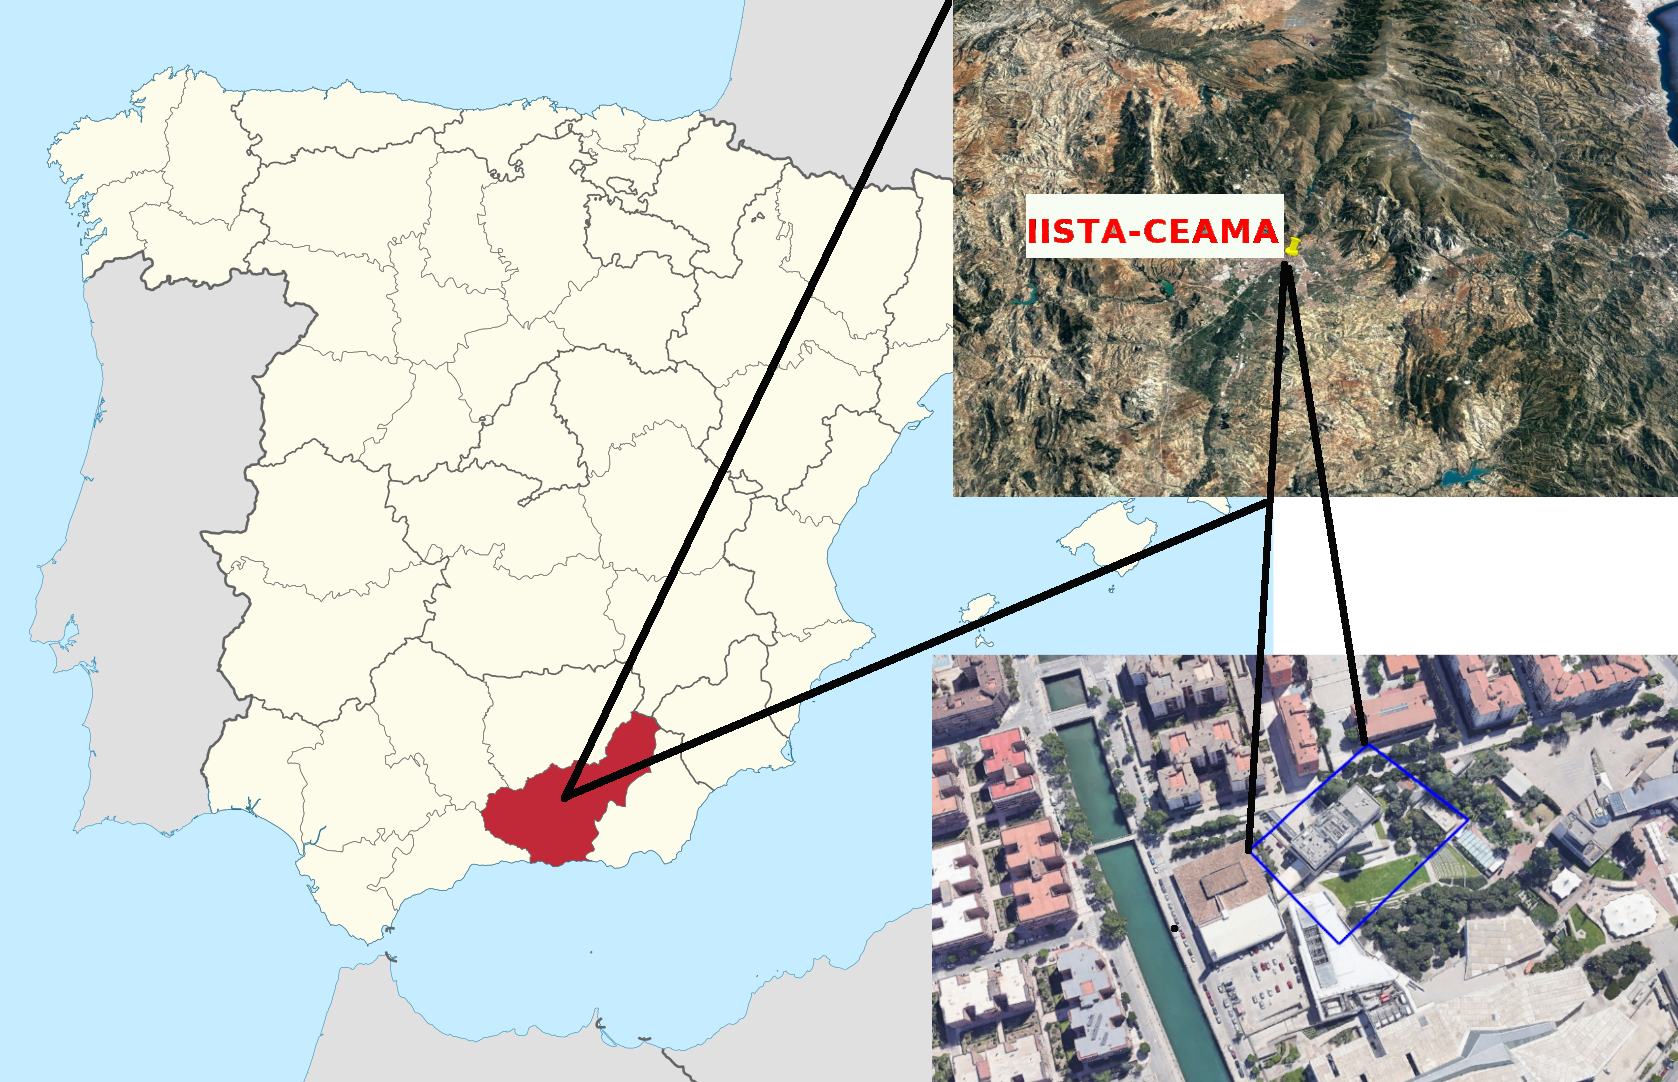
\includegraphics[width=1.\textwidth]{../phd_clouds/figures/Granada_station2.png}
      \caption{Geographic location of the ACTRIS CCRES Granada station. Red area is the province of granada, while blue poligon indicates the station facility, the Andalusian Institute for Earth System Research. Image adapted from \href{https://en.wikipedia.org/wiki/Province_of_Granada}{wikipedia} with Google Earth software.}
      \label{fig:granada_station}
\end{figure}

The Cloudnet processed data was determined by a synergy between a RPG-HATPRO radiometer, a CHM15k ceilometer, a RPG-FMCW 94 GHz cloud Doppler radar and the European model ECMWF (an acronym for European Centre for Medium-Range Weather Forecasts). These instruments have been continuously operated since 2018, and their data has been processed by the CloudnetPy \cite{Illingworth2007XXX}, performing reflectivity attenuation correction, error estimation and quality flag assignment. Particularly, attenuation corrections assists in prevention misclassification of atmospheric elements through liquid water content (LWC) estimation. This variable is obtained by cloud boundaries provided by lidar and radar synergy, and radiometer liquid water path (LWP) \cite{AlbreachXXX}. As a result, uncertainties retrieving LWP during a raining event can be high enough to frustrate attenuation corrections. Consequently, rain events were exclude from cloud analysis in the section \ref{XXX}, reducing misclassification occurence.

Processed data were sampled in a common grid with time resoltion of 30\,s, and height bins according to cloud radar range resolution, which differ according to radar chirp table configuration. Figure \ref{fig:radar_vertical_res} displays changes in the radar vertical bin size across dataset time serie, and table \ref{tab:instrument_info} associate bin sizes with their respective height intervals. This table also gives operational information of instruments at Granada site and their main post-processed variables. Differently, microwave radiometer humidity and temperature profiles were not processed by CloudnetPy, but were provided by its own manufacturing software.
High level data included in the analysis were target classification, liquid water path (LWP) and ice water path (IWP), where target classification apportioned to classify cloud layers as explained in section \ref{sec:XXX}. The classification method was adapted from \cite{PirloagaXXX} and \cite{NokomovaXXX}. 

\begin{figure}[htbp]
      \centering
      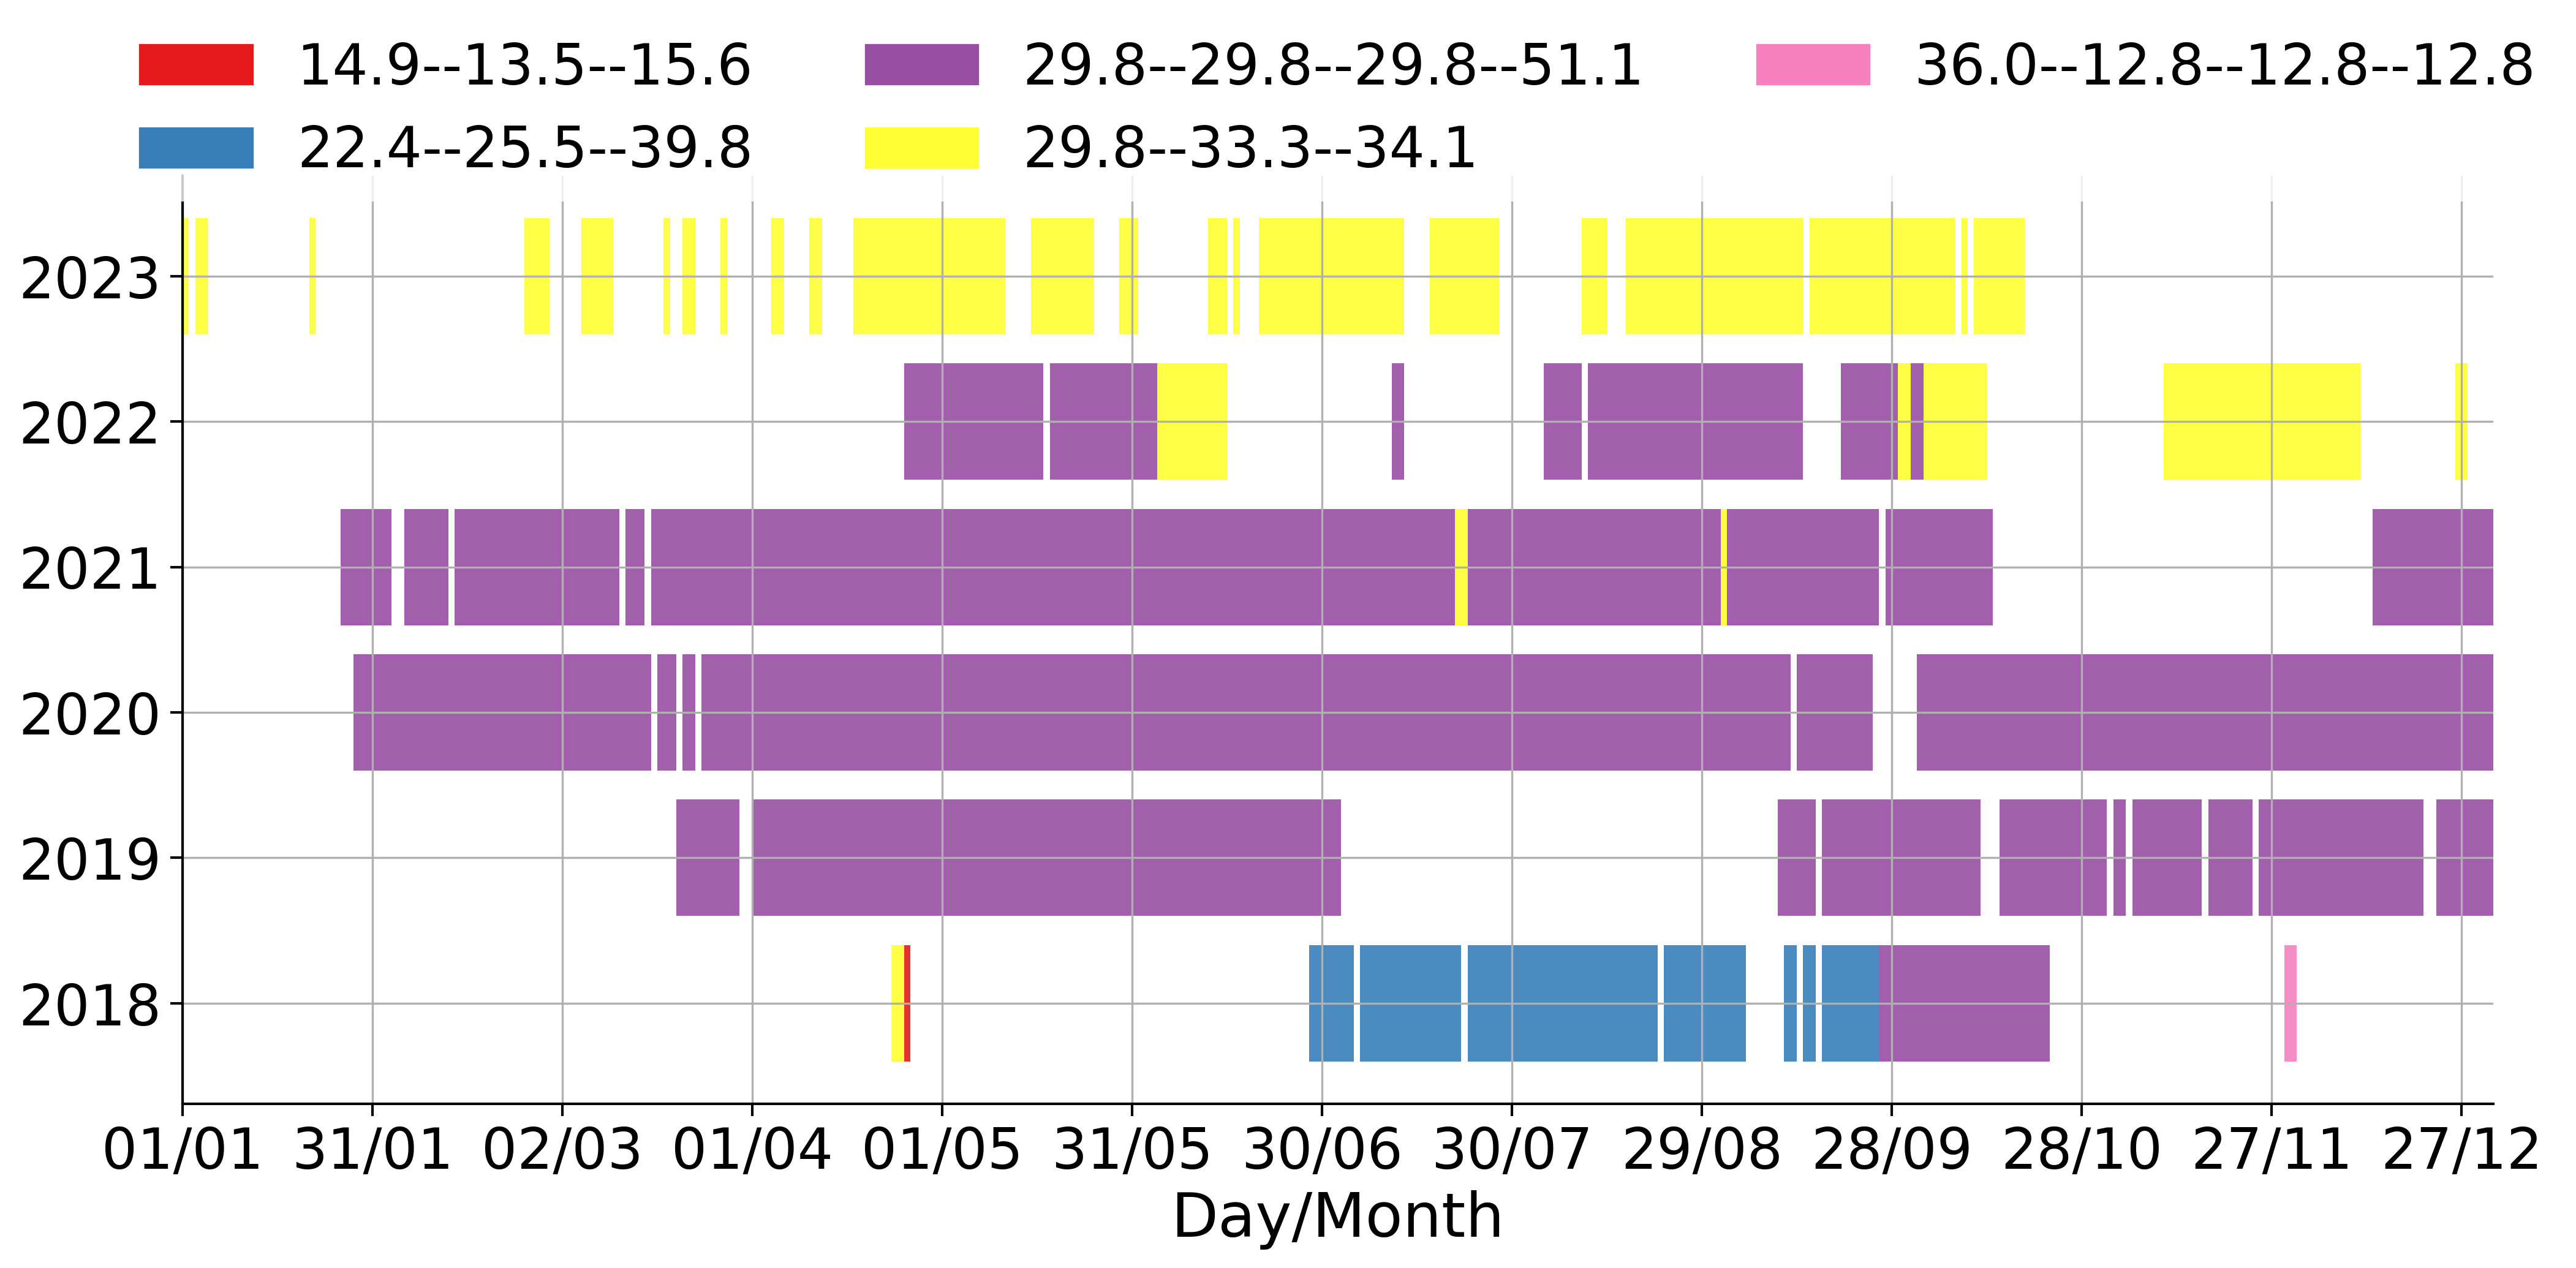
\includegraphics[width=1.\textwidth]{../phd_clouds/figures/chirp_intervals.png}
      \caption{Overview of cloud radar vertical bin sizes depending chirp table configuration.}
      \label{fig:radar_vertical_res}
\end{figure}

\begin{table}[htbp]
\caption{This is a sample table caption and table layout.}\label{tab:instrument_info}
\begin{tabular}{llcl}
\toprule
\textbf{Instrument}                                                                         & \textbf{Height resolution (heigh interval) (m)}                                                                   & \textbf{\begin{tabular}[c]{@{}c@{}}Integration \\ time (s)\end{tabular}} & \textbf{Variables}                                                                                                                                                      \\ \midrule
\multirow{5}{*}{\begin{tabular}[c]{@{}l@{}}FMCW 94 GHz Cloud \\ Doppler Radar\end{tabular}} & 14.9 (100-1200), 13.5 (1200-4400), 15.5 (4400-10000)                                                              & 1.10                                                                     & \multirow{5}{*}{\begin{tabular}[c]{@{}l@{}}Mean Doppler vellocity (m/s) \\ Reflectivity (dBz) \\ Linear depolarisation ratio (dB) \\ Spectral width (m/s)\end{tabular}} \\ 
                                                                                            & 22.4 (100-924), 25.6 (924-8455), 39.7 (8455-12000)                                                                & 3.2                                                                      &                                                                                                                                                                         \\ 
                                                                                            & \begin{tabular}[c]{@{}l@{}}29.8 (100-1200), 29.8 (1200-4900), 29.8 (4900-8500), \\ 51.1 (8500-13500)\end{tabular} & 3.57                                                                     &                                                                                                                                                                         \\ 
                                                                                            & 29.8 (100-1200), 33.3 (1200-5500), 34.1 (5500-11000)                                                              & 3.26                                                                     &                                                                                                                                                                         \\
                                                                                            & \begin{tabular}[c]{@{}l@{}}36 (180-1476), 12.8 (1476-3998), 12.8 (3998-8158), \\ 12.8 (8158-1200)\end{tabular}    & 2.81                                                                     &                                                                                                                                                                         \\ \hline
\multirow{3}{*}{MWR RPG HATPRO}                                                             & \multicolumn{1}{c}{200 (0-2000), 400 (2000-5000), 800 (5000-10000)}                                              & 10                                                                       & Humidity profiles (g m$^{-3}$)                                                                                                                                          \\
                                                                                            & \multicolumn{1}{c}{50 (0-1200), 200 (1200-5000), 400 (5000-10000)}                                               & 10                                                                       & Temperature profiles (K)                                                                                                                                                \\ 
                                                                                            & \multicolumn{1}{c}{--}                                                                                           & 2                                                                        & LWP, IWP (kg m$^{-2}$)                                                                                                                                                  \\ \hline
\begin{tabular}[c]{@{}l@{}}CHM15k Nimbus \\ Ceilometer (1064 nm)\end{tabular}               & \multicolumn{1}{c}{15}                                                                                           & 15                                                                       & \begin{tabular}[c]{@{}l@{}}Attenuated backscatter \\ coefficient (sr$^{-1}$ m$^{-1} $)\end{tabular}                                                                     \\ \bottomrule
\end{tabular}
\end{table}

Typical variables of each instruments in table \ref{tab:instrument_info} in Granada station is shown in Figure \ref{XXX}. The corresponding instrument is depicted on the right side.


\begin{figure}[htbp]
      \centering
      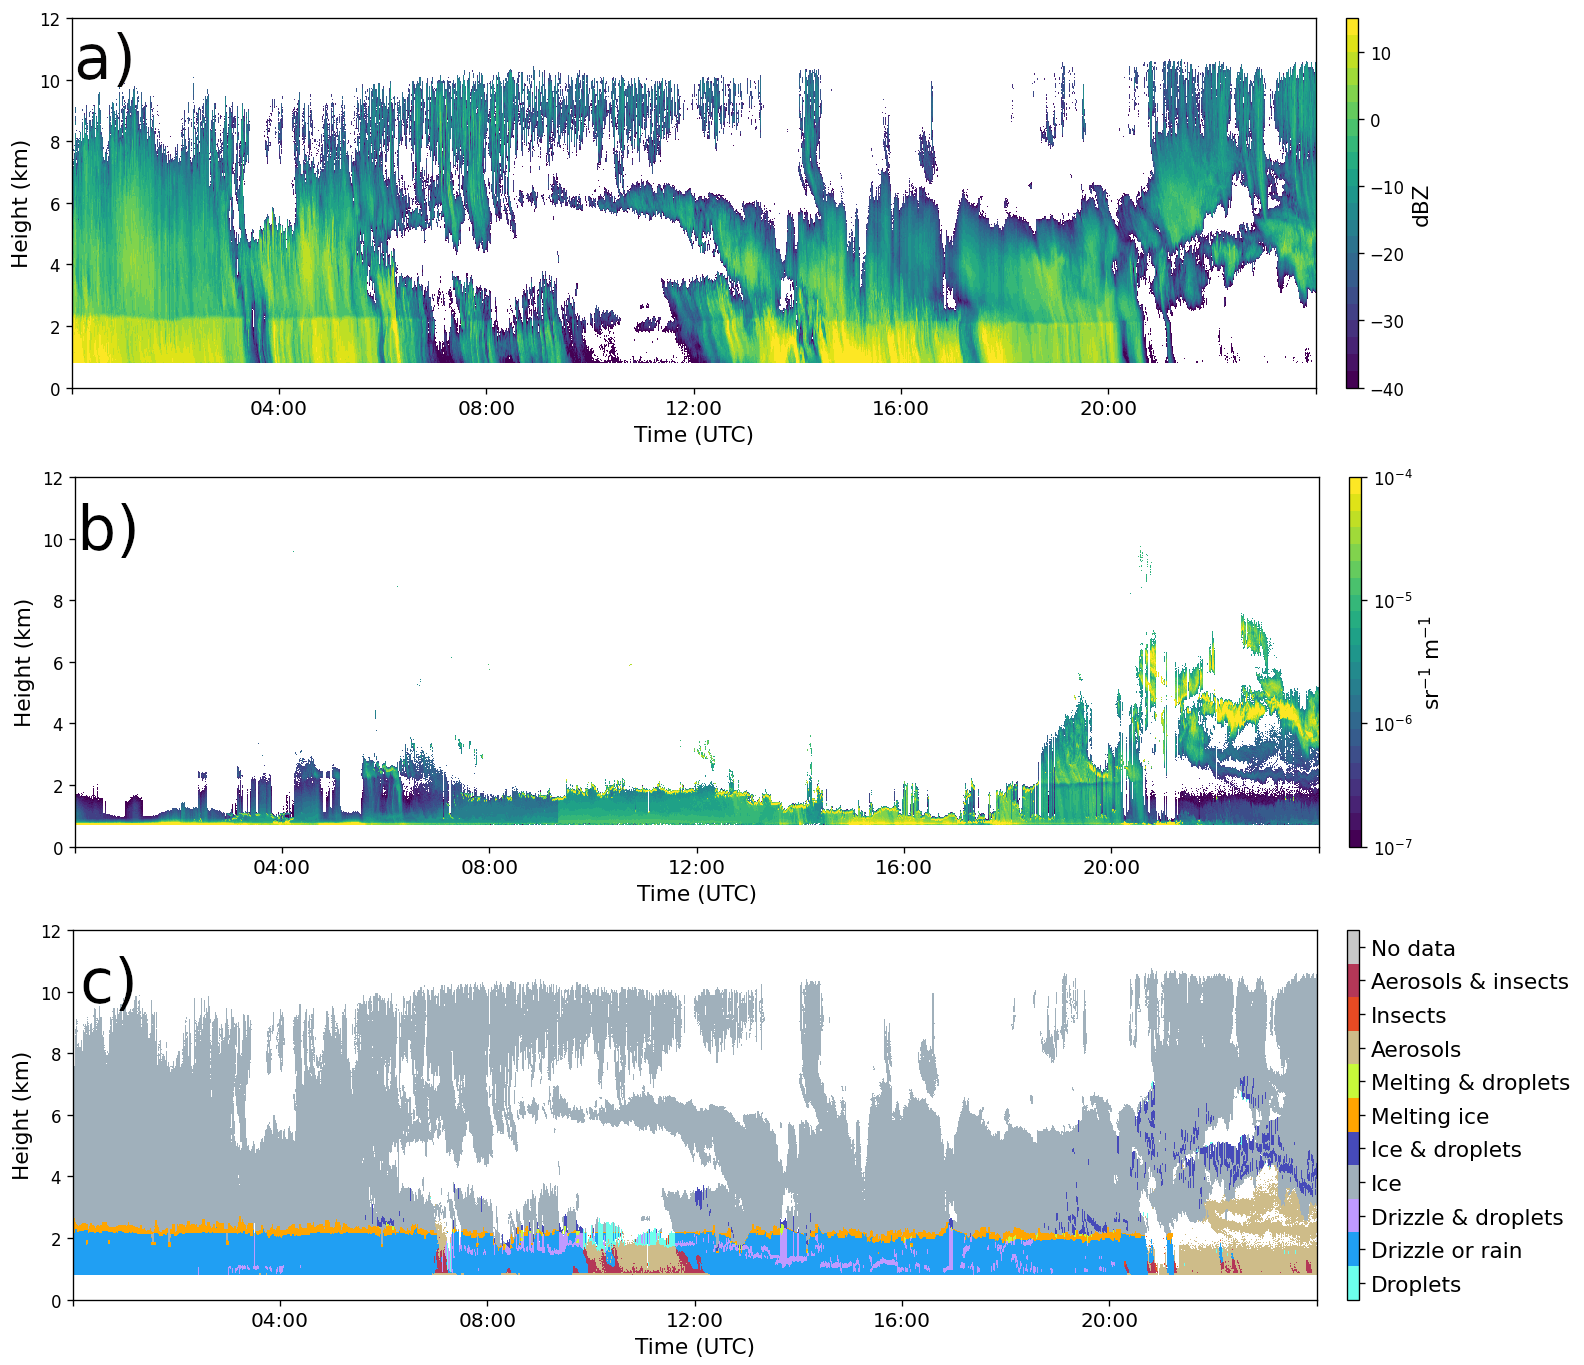
\includegraphics[width=1.\textwidth]{../phd_clouds/figures/cloudnet_products.png}
      \caption{Should change figure - Reflectivity, Att. backscatter coeff and LWP}
      \label{fig:product_vs_intrument}
\end{figure}

\subsection{Cloudnet particle classification scheme}

Target classification product assigns an integer ranging from 0 to 10 at each pixel in the Cloudnet processed grid. Each number are related to atmospheric elements in the following order: clear sky, droplets, drizzle or rain, drizzle \& droplets, ice, ice \& droplets, melting ice, melting \& droplets, aerosol, insects, aerosol \& insect. These targets were determined through radar and lidar variables in combination with thermodynamic profiles from the ECMWF model. In particular, wet bulb temperature (T$_w$) profiles is used to establish warm and cold regions to classify liquid and ice hydrometeors. For instance, ice and melting particles can only exist in cold regions, in other words, when T$_w$ < 0. Further, liquid droplets boundaries were resolved with lidar attenuated backscatter coefficient ($\beta$), and radar reflectivity. The first is sensible to small liquid droplets present in cloud base, being used to identify lower limits of droplet layers and also upper limits when there is no radar reflectivity above the heigh lidar signal was totally attenuated. In addition, liquid layers respect a threshold of T$_w$ < -40 $^{\circ}$C, since it is not possible to keep water in liquid phase bellow that temperature. Hence, liquid droplets assigned as falling were classified as drizzle or rain droplets, where falling is attributed through radar echos analysis once particles boundary were already determined. Therefore, falling cold particle were just classified as ice, without distinguishing ice from precipitating ice. Next, melting layers were identified at the height of maximum wet bulb temperature divergence. Pixels with divergence surpassing 0.0075 s$^{-1}$ within 150 m of height deviation were also classified as "melting". Furthermore, more than one class of particle can be settled in the same pixel, allowing the identification of mixed phase hydrometeors, like ice coexisting with supercooled liquid droplets and melting ice particles coexisting with cloud liquid droplets. A more detailed description of particle apportionment of Cloudnet algorithm can be found on \cite{XXX}. 


\subsection{Assortment algorithm}\label{sec:classification_algorithm}

The assortment algoritm classifies groups of hydrometeors and cloud layers. In terms of hydrometeors, this algorithm generate masks of hydrometeor occurence for 3 groups: liquid, ice and "total", where liquid class encompass all possible liquid pixels, which are "droplets", "drizzle or rain" and "drizzle \& droplets". Ice encompass only "ice" pixels, and total is all possible hydrometeors, whic are "droplets", "drizzle or rain", "drizzle \& droplets", "ice", "ice \& droplets", "melting ice" and "melting \& droplets".

Subsequently, cloud layers in atmospheric column were classified trought pixel sequence inquiry. These pixels sequences were devided in the following 5 groups according to \cite{PirloagaXXX}: liquid, ice, mixed phase, liquid with precipitation and mixed phase with precipitation. Specifically, liquid clouds were assigned as any combination of "droplets" and "drizzle \& droplets" pixels. Ice clouds were assigned when only "ice" pixel sequence was encountered. As well as, mixed phase clouds were assigned with any combination of "droplets", "ice", "ice \& droplets", "melting ice", "melting \& droplets", "drizzle and droplets" pixels. Precipitation cases were classified wheter at least one pixel of "drizzle or rain" is found below liquid and mixed phase clouds. Diferent from previous studies, a threshold of 20 bins (256-1022 m) bellow cloud was set to reject precipitation events, assuming that rain droplets are not falling from the actual cloud layer. In all cases, for being considered a cloud layer, a minimun sequence of 3 cloud pixels (38-153 m) (as \citep{NomokovaXXX}) must be satisfied, in addition to a minimun sequence of 5 pixels (64-255 m) of "Clear sky", "Aerosol", "Insect" and "Arosol \& insect" to separate multilayers. Therefore, free hydrometeor layers in the neghborhood of the cloud allowed the identification of cloud base and top. Nevertheless, thresholds here were based on \cite{Pirloaga and NokomovaXXX}, but theses values are not currently well defined, their determination has been guided by empirical experience.

\section{Thermodinamic conditions}


\begin{figure}[htbp]
      \centering
      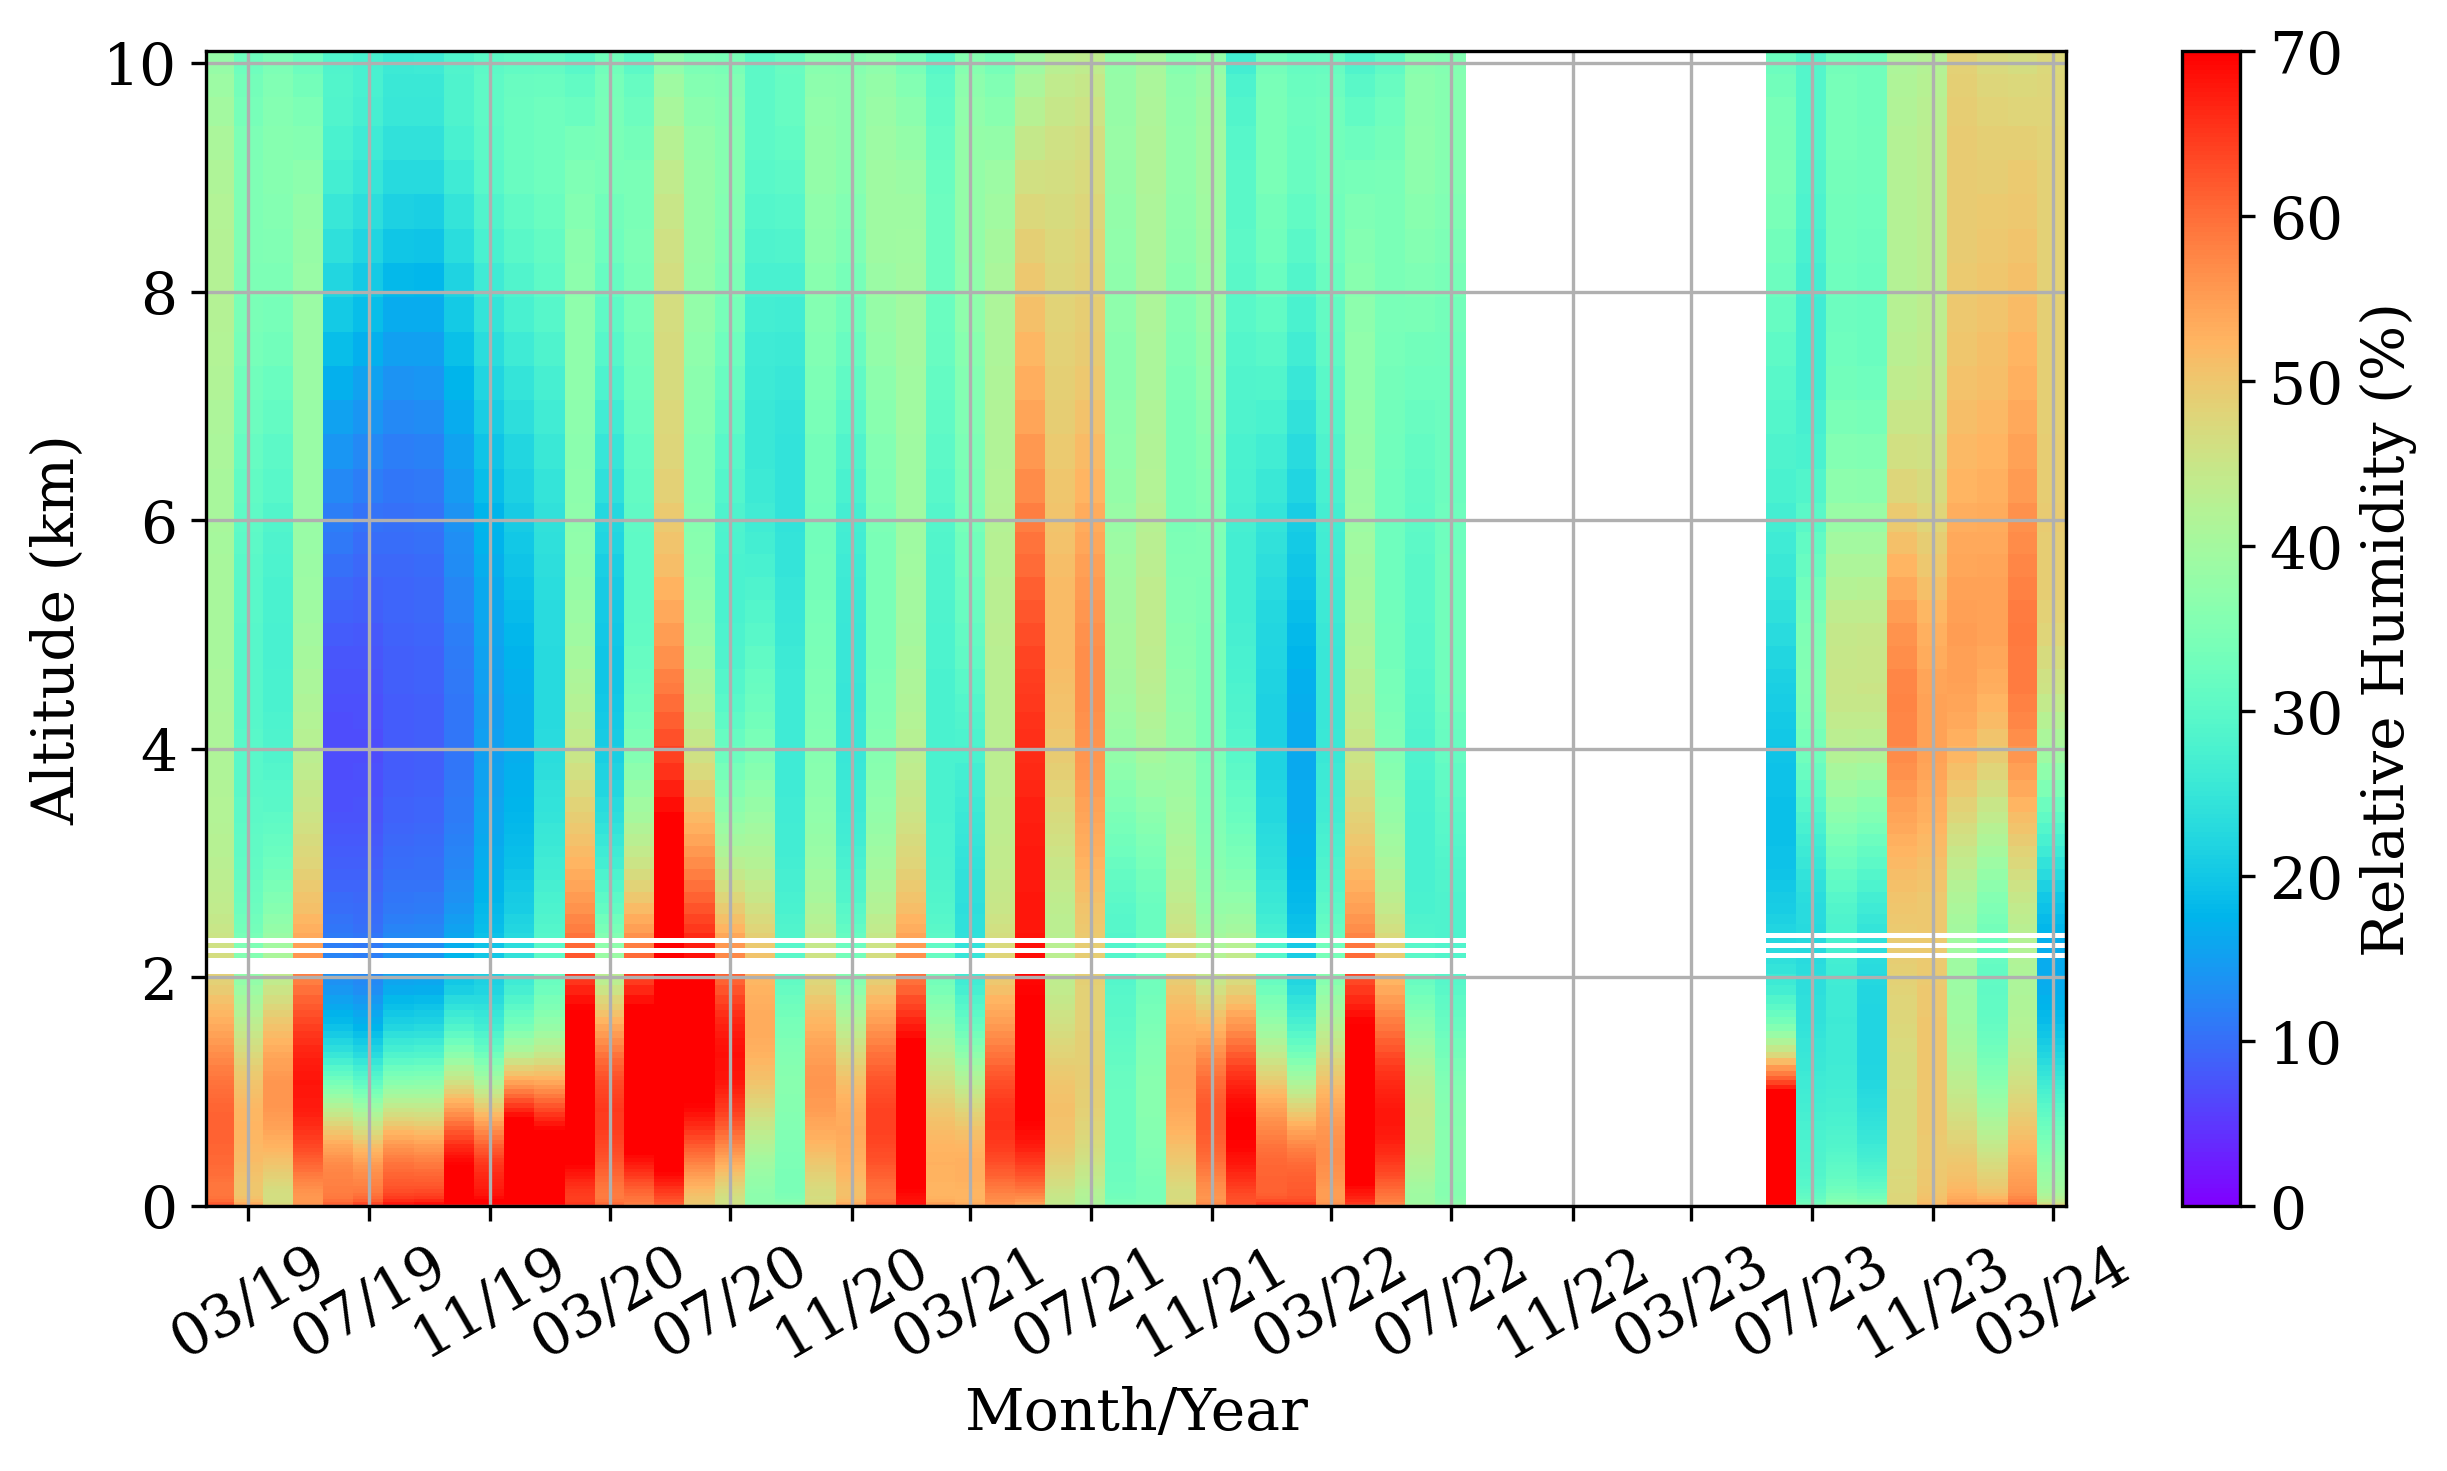
\includegraphics[width=1.\textwidth]{../phd_clouds/figures/mwr_time_series_RH.png}
      \caption{Should change figure - Reflectivity, Att. backscatter coeff and LWP}
      \label{fig:temo}
\end{figure}

\section{Hydrometeor characteristics}

A first conception about clouds spacial-temporal distribution can be acessed with the hydrometeor frequency of occurence. Hence, figure \ref{fig:hydro_occurence} shows the frequency of occurence for liquid, ice and all hydrometeors. In terms of liquid hydrometeors, a notably concentration below 2\,km can be observed in both panels of figure~\ref{fig:hydro_occurence}.a, where left panel shows the time evolution of montly vertical frequency of occurence, while the right panel shows the mean profile through the entire dataset. On the contrary, ice particles (figure figure~\ref{fig:hydro_occurence}.b) shows a completely different behavior, with a spreader distribution along the vertical, with slight maxima in 2\,km and 8\,km viwed in the mean profile, and a clear seasonality, with low frequencies in summer/fall and higher frequency in winter/spring. 

\begin{figure}[htbp]
      \centering
      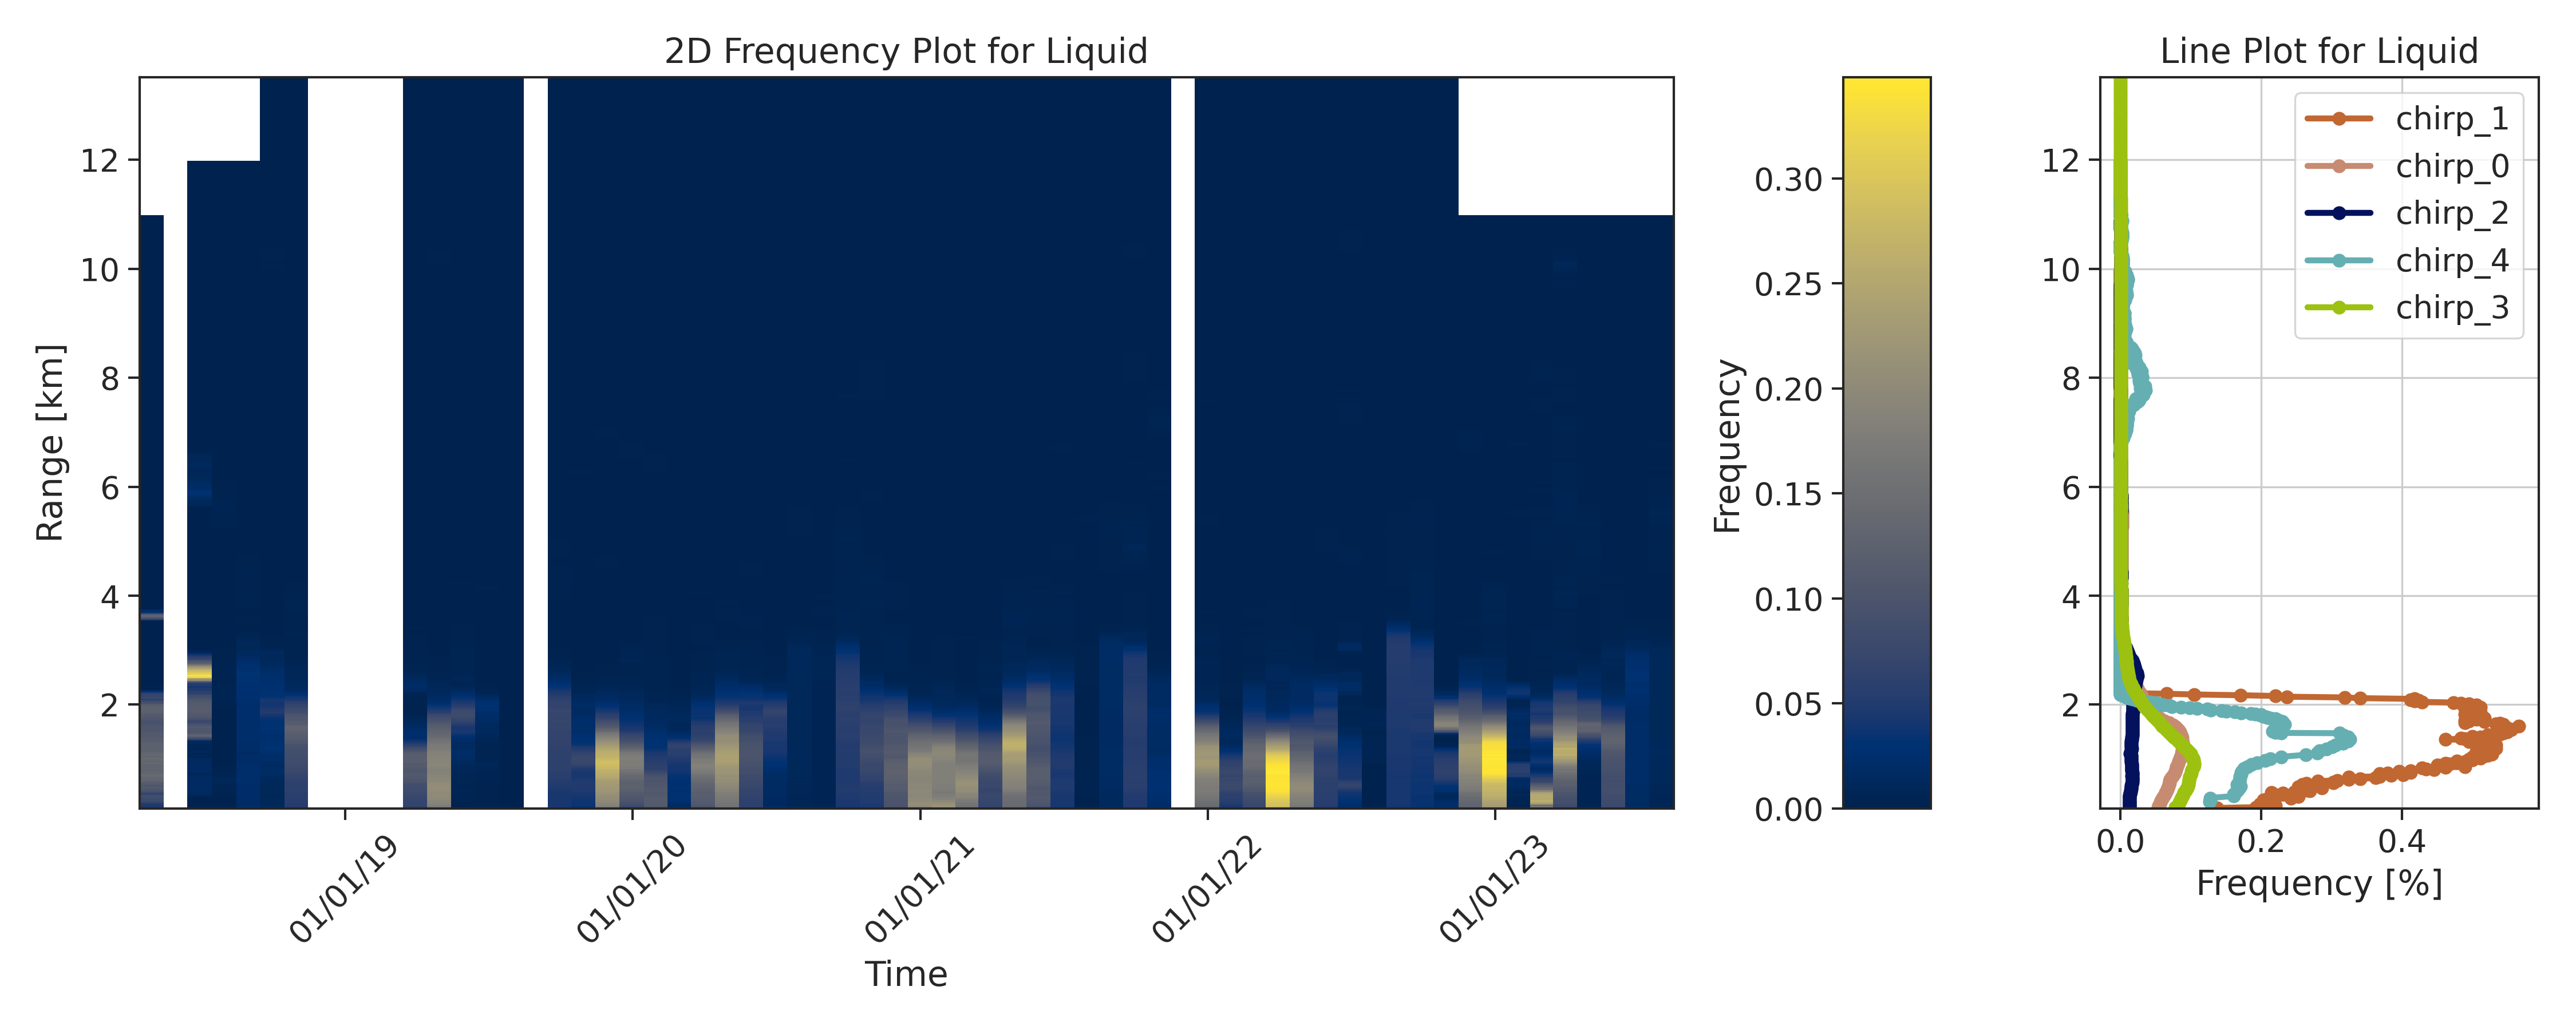
\includegraphics[width=1.\textwidth]{../phd_clouds/figures/Liquid_2d_histogram_hydrometeors}
      \caption{Should change figure - Reflectivity, Att. backscatter coeff and LWP}
      \label{fig:hydro_occurence}
\end{figure}



\section{Cloud properties evaluation}
















% The other hydrometeors follows a complex

% height of maximum divergence within a specified temperature range (Tw). Pixels with divergence surpassing 0.0075 s^(-1) within 150 m of this height are classified as "melting" 

% identified with  particles with falling velocity identified with the mean radar Doppler velocity, are likely drizzle or rain droplets . 


% For hydrometeors, bit fields are droplet, cold, melting and falling. The droplet bit uses lidar attenuated backscatter coefficient and radar reflectivity to determine liquid boundaries. 

% First, cold and melting bits were assigned using model wet bulb temperature, and Doppler velocity for assessment assurance. Than, droplet bit uses lidar backscatter coefficient to determine liquid boundaries, and radar reflectivity to assure lidar signal was not extinguished before radar cloud top. In addition cold bit is used to resolve which cloud top is more likely, and a threshold of -40 $^{\circ}$ C was defined to reset liquid bits. For the profiles without liquid droplets.

% Next, Falling bit and insect focuses on profiles without liquid water droplets and lacking radar echo in the lowest sub-zero pixel, categorizing finite radar reflectivity as "falling" based on rain detection. For profiles with liquid water droplets, single-pixel liquid clouds are considered, distinguishing precipitation from insects. 
 
% The analysis initially focuses on profiles without liquid water droplets and lacking radar echo in the lowest sub-zero pixel, categorizing finite radar echoes as "falling" or "insects" based on rain detection. Then liquid water droplets were identified with cold bit defined before.


% --------------------------------------------------------------
% radar used to detect rain, drizzle, ice and insects.
% water vapor and molecular oxygen atenuation: estimated with termodinamic variables from models. Atenuation of 1-3 dB to cirrus altitude, at 94 GHz

% Liquid atenuation: LWC with radiometer LWP and cloud boundaries using lidar and radar
% Atenuation of 4.5 for LWP of 500 gm-2 at 94 GHz

% No attenuation when is raining, uncertanty retrieveing LWP

% lidar used to detect high concentrations of cloud droplets and aerosol 
% - high lidar backscatter identify supercooled liquid layers, and step change in doppler velocity in the 0C (model) indicate melting ice

% This classification mask is shown in figure XXX and was used as an entry to an algorithm of cloud profile classification, explained in detail in section XXX. 
% % --------------------------------------------------------------

\subsection{HEADING}
TEXT


\subsubsection{HEADING}
TEXT


\conclusions  %% \conclusions[modified heading if necessary]
TEXT

%% The following commands are for the statements about the availability of data sets and/or software code corresponding to the manuscript.
%% It is strongly recommended to make use of these sections in case data sets and/or software code have been part of your research the article is based on.

\codeavailability{TEXT} %% use this section when having only software code available


\dataavailability{TEXT} %% use this section when having only data sets available


\codedataavailability{TEXT} %% use this section when having data sets and software code available


\sampleavailability{TEXT} %% use this section when having geoscientific samples available


\videosupplement{TEXT} %% use this section when having video supplements available


\appendix
\section{}    %% Appendix A

\subsection{}     %% Appendix A1, A2, etc.


\noappendix       %% use this to mark the end of the appendix section. Otherwise the figures might be numbered incorrectly (e.g. 10 instead of 1).

%% Regarding figures and tables in appendices, the following two options are possible depending on your general handling of figures and tables in the manuscript environment:

%% Option 1: If you sorted all figures and tables into the sections of the text, please also sort the appendix figures and appendix tables into the respective appendix sections.
%% They will be correctly named automatically.

%% Option 2: If you put all figures after the reference list, please insert appendix tables and figures after the normal tables and figures.
%% To rename them correctly to A1, A2, etc., please add the following commands in front of them:

\appendixfigures  %% needs to be added in front of appendix figures

\appendixtables   %% needs to be added in front of appendix tables

%% Please add \clearpage between each table and/or figure. Further guidelines on figures and tables can be found below.



\authorcontribution{TEXT} %% this section is mandatory

\competinginterests{TEXT} %% this section is mandatory even if you declare that no competing interests are present

\disclaimer{TEXT} %% optional section

\begin{acknowledgements}
TEXT
\end{acknowledgements}




%% REFERENCES

%% The reference list is compiled as follows:

\begin{thebibliography}{}

\bibitem[AUTHOR(YEAR)]{LABEL1}
REFERENCE 1

\bibitem[AUTHOR(YEAR)]{LABEL2}
REFERENCE 2

\end{thebibliography}

%% Since the Copernicus LaTeX package includes the BibTeX style file copernicus.bst,
%% authors experienced with BibTeX only have to include the following two lines:
%%
%% \bibliographystyle{copernicus}
%% \bibliography{example.bib}
%%
%% URLs and DOIs can be entered in your BibTeX file as:
%%
%% URL = {http://www.xyz.org/~jones/idx_g.htm}
%% DOI = {10.5194/xyz}


%% LITERATURE CITATIONS
%%
%% command                        & example result
%% \citet{jones90}|               & Jones et al. (1990)
%% \citep{jones90}|               & (Jones et al., 1990)
%% \citep{jones90,jones93}|       & (Jones et al., 1990, 1993)
%% \citep[p.~32]{jones90}|        & (Jones et al., 1990, p.~32)
%% \citep[e.g.,][]{jones90}|      & (e.g., Jones et al., 1990)
%% \citep[e.g.,][p.~32]{jones90}| & (e.g., Jones et al., 1990, p.~32)
%% \citeauthor{jones90}|          & Jones et al.
%% \citeyear{jones90}|            & 1990



%% FIGURES

%% When figures and tables are placed at the end of the MS (article in one-column style), please add \clearpage
%% between bibliography and first table and/or figure as well as between each table and/or figure.

% The figure files should be labelled correctly with Arabic numerals (e.g. fig01.jpg, fig02.png).


%% ONE-COLUMN FIGURES

%%f
%\begin{figure}[t]
%\includegraphics[width=8.3cm]{FILE NAME}
%\caption{TEXT}
%\end{figure}
%
%%% TWO-COLUMN FIGURES
%
%%f
%\begin{figure*}[t]
%\includegraphics[width=12cm]{FILE NAME}
%\caption{TEXT}
%\end{figure*}
%
%
%%% TABLES
%%%
%%% The different columns must be seperated with a & command and should
%%% end with \\ to identify the column brake.
%
%%% ONE-COLUMN TABLE
%
%%t
%\begin{table}[t]
%\caption{TEXT}
%\begin{tabular}{column = lcr}
%\tophline
%
%\middlehline
%
%\bottomhline
%\end{tabular}
%\belowtable{} % Table Footnotes
%\end{table}
%
%%% TWO-COLUMN TABLE
%
%%t
%\begin{table*}[t]
%\caption{TEXT}
%\begin{tabular}{column = lcr}
%\tophline
%
%\middlehline
%
%\bottomhline
%\end{tabular}
%\belowtable{} % Table Footnotes
%\end{table*}
%
%%% LANDSCAPE TABLE
%
%%t
%\begin{sidewaystable*}[t]
%\caption{TEXT}
%\begin{tabular}{column = lcr}
%\tophline
%
%\middlehline
%
%\bottomhline
%\end{tabular}
%\belowtable{} % Table Footnotes
%\end{sidewaystable*}
%
%
%%% MATHEMATICAL EXPRESSIONS
%
%%% All papers typeset by Copernicus Publications follow the math typesetting regulations
%%% given by the IUPAC Green Book (IUPAC: Quantities, Units and Symbols in Physical Chemistry,
%%% 2nd Edn., Blackwell Science, available at: http://old.iupac.org/publications/books/gbook/green_book_2ed.pdf, 1993).
%%%
%%% Physical quantities/variables are typeset in italic font (t for time, T for Temperature)
%%% Indices which are not defined are typeset in italic font (x, y, z, a, b, c)
%%% Items/objects which are defined are typeset in roman font (Car A, Car B)
%%% Descriptions/specifications which are defined by itself are typeset in roman font (abs, rel, ref, tot, net, ice)
%%% Abbreviations from 2 letters are typeset in roman font (RH, LAI)
%%% Vectors are identified in bold italic font using \vec{x}
%%% Matrices are identified in bold roman font
%%% Multiplication signs are typeset using the LaTeX commands \times (for vector products, grids, and exponential notations) or \cdot
%%% The character * should not be applied as mutliplication sign
%
%
%%% EQUATIONS
%
%%% Single-row equation
%
%\begin{equation}
%
%\end{equation}
%
%%% Multiline equation
%
%\begin{align}
%& 3 + 5 = 8\\
%& 3 + 5 = 8\\
%& 3 + 5 = 8
%\end{align}
%
%
%%% MATRICES
%
%\begin{matrix}
%x & y & z\\
%x & y & z\\
%x & y & z\\
%\end{matrix}
%
%
%%% ALGORITHM
%
%\begin{algorithm}
%\caption{...}
%\label{a1}
%\begin{algorithmic}
%...
%\end{algorithmic}
%\end{algorithm}
%
%
%%% CHEMICAL FORMULAS AND REACTIONS
%
%%% For formulas embedded in the text, please use \chem{}
%
%%% The reaction environment creates labels including the letter R, i.e. (R1), (R2), etc.
%
%\begin{reaction}
%%% \rightarrow should be used for normal (one-way) chemical reactions
%%% \rightleftharpoons should be used for equilibria
%%% \leftrightarrow should be used for resonance structures
%\end{reaction}
%
%
%%% PHYSICAL UNITS
%%%
%%% Please use \unit{} and apply the exponential notation


\end{document}
